% coding:utf-8

\section{Layout}
Die Platine wird direkt an den XLR-Stecker vom Typ NC3MD-V von Neutrik angelötet. Die Verbindung zu einem Arduino erfolgt über eine Steckerleiste. Alle übrigen Bauteile sind in SMD mit der Baugrösse 0805 bzw. 1206 ausgeführt. Die Grösse der Platine ist auf den Steckverbinder angepasst, so dass dieser mit der angelöteten Platine montiert werden kann. 
\begin{figure}[h!]
	\centering
	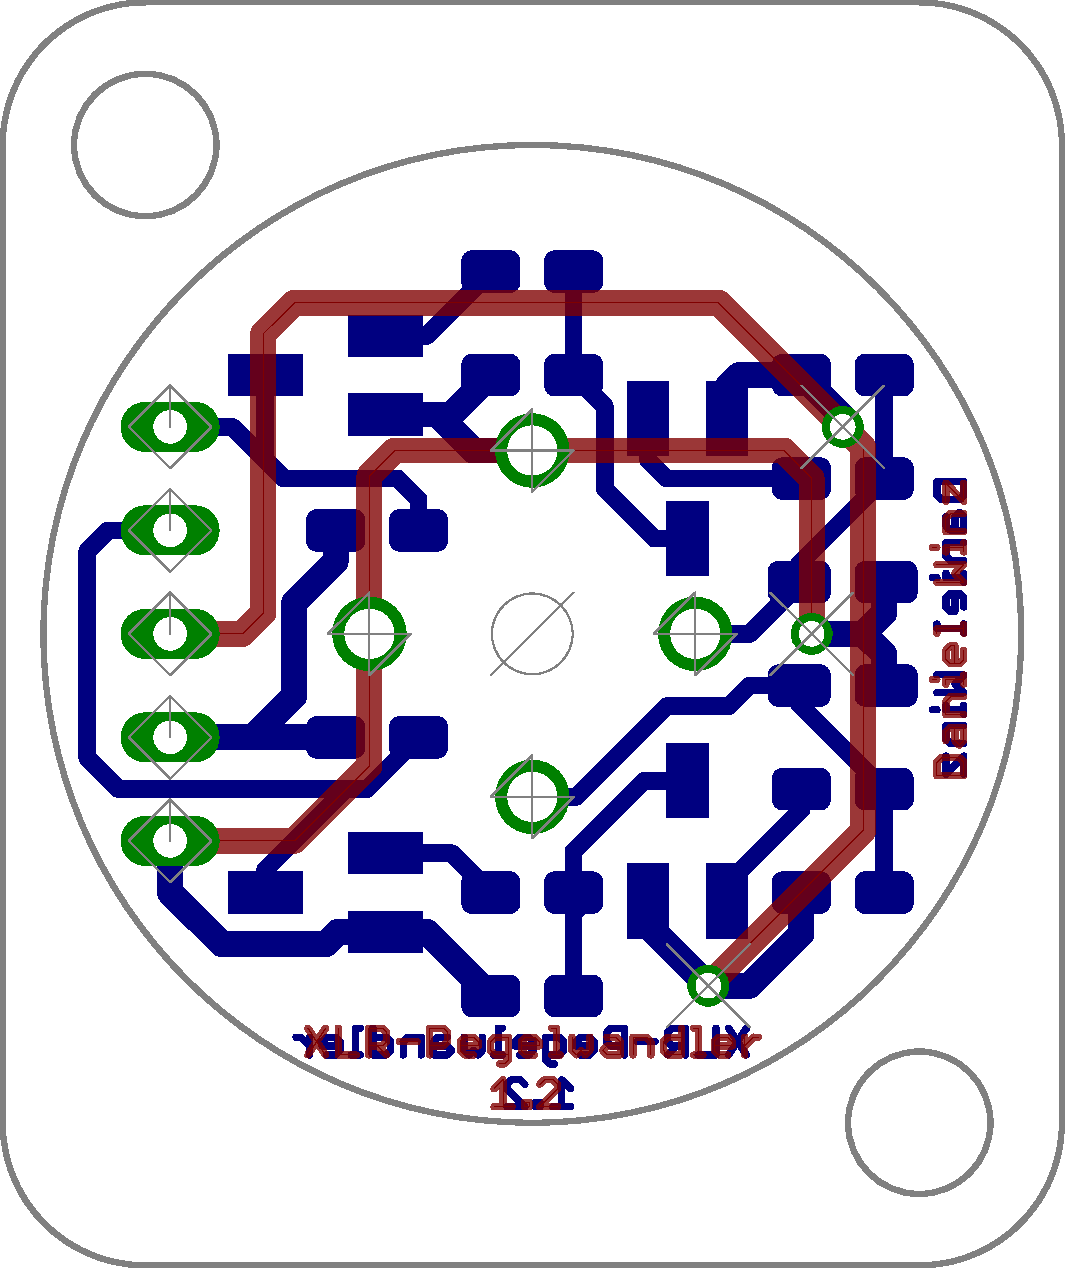
\includegraphics[scale=\layscale]{fig/xlr_pegelwandler_v_1_2_lay_transp.pdf}
	\caption{Layout}
	\label{lay:pegw}
\end{figure}
